\chapter{Installation and First Use}
\section{Introduction}

The following chapter presents how to download and configure ASK on the user's workstation.

\section{Download}

Download ASK through the Git version control system:

\begin{minted}{bash}
$ git clone https://code.google.com/p/adaptive-sampling-kit/
\end{minted}

The previous command retrieves the current stable version of ASK. To switch to the development version type:

\begin{minted}{bash}
$ cd ask
$ git checkout develop
\end{minted}

\section{Configuration}

Before using ASK, make sure all its dependencies are satisfied:

\begin{itemize}
	\item Python: at least version 2.6
\end{itemize}

\begin{itemize}
	\item R
\end{itemize}

\begin{itemize}
	\item Libraries: python-numpy, python-scipy and python-argparse
\end{itemize}

\begin{itemize}
	\item Optionally, nosetests, which is only needed to \hrefinternal{http:///wiki/Application\_Characterization:\_ASK:\_Chapter\_6:\_Support\#Running\_the\_Test\_Suite}{run the regression test suite}
\end{itemize}

In a Debian or Ubuntu system, use:

\begin{minted}{bash}
$ sudo apt-get install python2.6 r-base python-numpy python-scipy \
       python-argparse python-nose
\end{minted}

Ensure that R\_LIBS contains a writable directory. For example, add the following line to your \texttt{.bashrc}, or equivalent, file:
\begin{minted}{bash}
export R_LIBS=$HOME/.R-libs:$R_LIBS
\end{minted}

and create the directory with:
\begin{minted}{bash}
$ mkdir $HOME/.R-libs/
\end{minted}

Once the dependencies are installed and R\_LIBS configured, enter ASK's directory and execute the \texttt{configure} script.

\begin{minted}{bash}
$./configure
Checking if R is installed
Checking if python is installed
All the dependencies are satisfied.
Building uniform sampling dynamic library (only needed for amart sampler module)
\end{minted}

The configure script makes sure all previous dependencies are properly installed.
It also retrieves a set of R modules from \href{http://cran.r-project.org/}{rcran}.
Therefore, before running this script, make sure the computer is connected to the internet.

ASK installation is self-contained: it does not install system-wide files. The \texttt{ask} binary can be run directly, or added to 
the PATH environment variable, eg. in bash:
\begin{minted}{bash}
cd ask/
export PATH=$PWD:$PATH
\end{minted}

The ASK directory contains the following subdirectories:

\begin{itemize}
	\item \texttt{common/}, contains common libraries
\end{itemize}

\begin{itemize}
	\item \texttt{examples/}, contains runable examples of ASK's usage
\end{itemize}

\begin{itemize}
	\item \texttt{tests/}, contains the \hrefinternal{http:///wiki/Application\_Characterization:\_ASK:\_Chapter\_6:\_Support\#Running\_the\_Test\_Suite}{test regression suite}
\end{itemize}

\begin{itemize}
	\item \texttt{bootstrap/}, contains the standard \hrefinternal{http:///wiki/Application\_Characterization:\_ASK:\_Chapter\_4:\_Standard\_Modules\#Bootstrap\_Modules}{Bootstrap modules}
\end{itemize}

\begin{itemize}
	\item \texttt{control/}, contains the standard \hrefinternal{http:///wiki/Application\_Characterization:\_ASK:\_Chapter\_4:\_Standard\_Modules\#Control\_Modules}{Control modules}
\end{itemize}

\begin{itemize}
	\item \texttt{model/}, contains the standard \hrefinternal{http:///wiki/Application\_Characterization:\_ASK:\_Chapter\_4:\_Standard\_Modules\#Model\_Modules}{Model modules}
\end{itemize}

\begin{itemize}
	\item \texttt{reporter/}, contains the standard \hrefinternal{http:///wiki/Application\_Characterization:\_ASK:\_Chapter\_4:\_Standard\_Modules\#Reporter\_Modules}{Reporter modules}
\end{itemize}

\begin{itemize}
	\item \texttt{sampler/}, contains the standard \hrefinternal{http:///wiki/Application\_Characterization:\_ASK:\_Chapter\_4:\_Standard\_Modules\#Sampler\_Modules}{Sampler modules}
\end{itemize}

\begin{itemize}
	\item \texttt{source/}, contains the standard \hrefinternal{http:///wiki/Application\_Characterization:\_ASK:\_Chapter\_4:\_Standard\_Modules\#Source\_Modules}{Source modules}
\end{itemize}

\begin{itemize}
	\item \texttt{utils/}, contains two scripts handling time series, described in \hrefinternal{http:///wiki/Application\_Characterization:\_ASK:\_Chapter\_3:\_Experiment\_Setup\#Analyzing\_the\_experiment}{Chapter 3}
\end{itemize}

\section{First Use}

Go into ASK's directory and type \texttt{ask -h} to get a brief summary of the command-line options.
\hrefinternal{http:///wiki/Application\_Characterization:\_ASK:\_Chapter\_3:\_Experiment\_Setup\#ASK\_invocation}{Chapter 3} explains in detail ASK's invocation.

Now, consider the \texttt{simple} experiment from the \texttt{examples} directory.

\begin{minted}{bash}
$ cd ask/; export PATH=$PWD:$PATH
$ cd examples/simple
$ ls 
gauss2D.data simple.conf
\end{minted}

Observe there are two files:

\begin{itemize}
	\item \texttt{Gauss2D.data} contains some measures:
\end{itemize}

\begin{minted}{rconsole}
-200 -200 -0.000670925255805024
-199 -200 -0.000694745225748637
-198 -200 -0.000719248849372865
-197 -200 -0.00074444881633483
-196 -200 -0.00077035776068282
-195 -200 -0.0007969882457312
-194 -200 -0.000824352748414127
-193 -200 -0.00085246364311948
-192 -200 -0.000881333185005384
-191 -200 -0.000910973492802606
...
\end{minted}

The last column represents the response; the first two columns are factors.

The above file contains an exhaustive measure of a design space inspired by an example from the article, \emph{tgp: An R package for Bayesian nonstationary, semiparametric nonlinear regression and design by treed gaussian process models. }, R. B. Gramacy, Journal of Statistical Software 2007: 

$$
f(x_1,x_2) = \frac{x_1}{100}.e^{-(\frac{x_1}{100})^2-(\frac{x_2}{100})^2} \textrm{ on } [-200:600] \times [-200:600]
$$

The design space has two factors, named x1 and x2 in the formula, and the response f(x1,x2).

\begin{itemize}
	\item \texttt{Simple.conf} contains the configuration of the experiment
\end{itemize}

The configuration file's first section, named factors, describes the factors of the experiment:

\begin{minted}{js}
"factors": [
  {"name": "x",
   "type": "integer",
   "range": {"min": -200, "max": 600}
  },
  {"name": "y",
   "type": "integer",
   "range": {"min": -200, "max": 600}
  }
]
\end{minted}

In the experiment, there are two factors called \textbf{x} and \textbf{y}, both of type \textbf{integer} and varying between -200 and 600, bounds included.

The second section, Modules, configures the ask modules involved in this experiment. The bootstrap module samples five hundred points random points, a general boosting machine (gbm) model is built and the 2D reporter plots the result. For a full discussion of module parameters please refer to \hrefinternal{http:///wiki/Application_Characterization:_ASK:_Chapter_3:_General_Usage}{Chapter 3}. 

To run the experiments, type:

\begin{minted}{bash}
$ ask simple.conf
Logging to default.log
Experiments finished normally
\end{minted}

The ask driver runs approximately for one minute and reports that the experiment finished without errors. While it is running, the \texttt{default.log} file tracks the driver's progress, the default.log file is created by default in the directory where ASK is invoked. ASK saves all the results into the default output directory \texttt{output/}:

\begin{minted}{bash}
$ ls output/
labelled00000.data  labelled.data  model00000.data  plot00000.png  
prediction00000.data
\end{minted}

Open the \texttt{plot00000.png} file in an image viewer, observe it shows two level plots:

\begin{itemize}
	\item The top one, shows the absolute error between the response model and the true response: white is better
\end{itemize}

\begin{itemize}
	\item The bottom one, shows the response model built using five hundred samples
\end{itemize}

\begin{itemize}
	\item The samples themselves are marked by the tiny circles
\end{itemize}

\begin{center}
  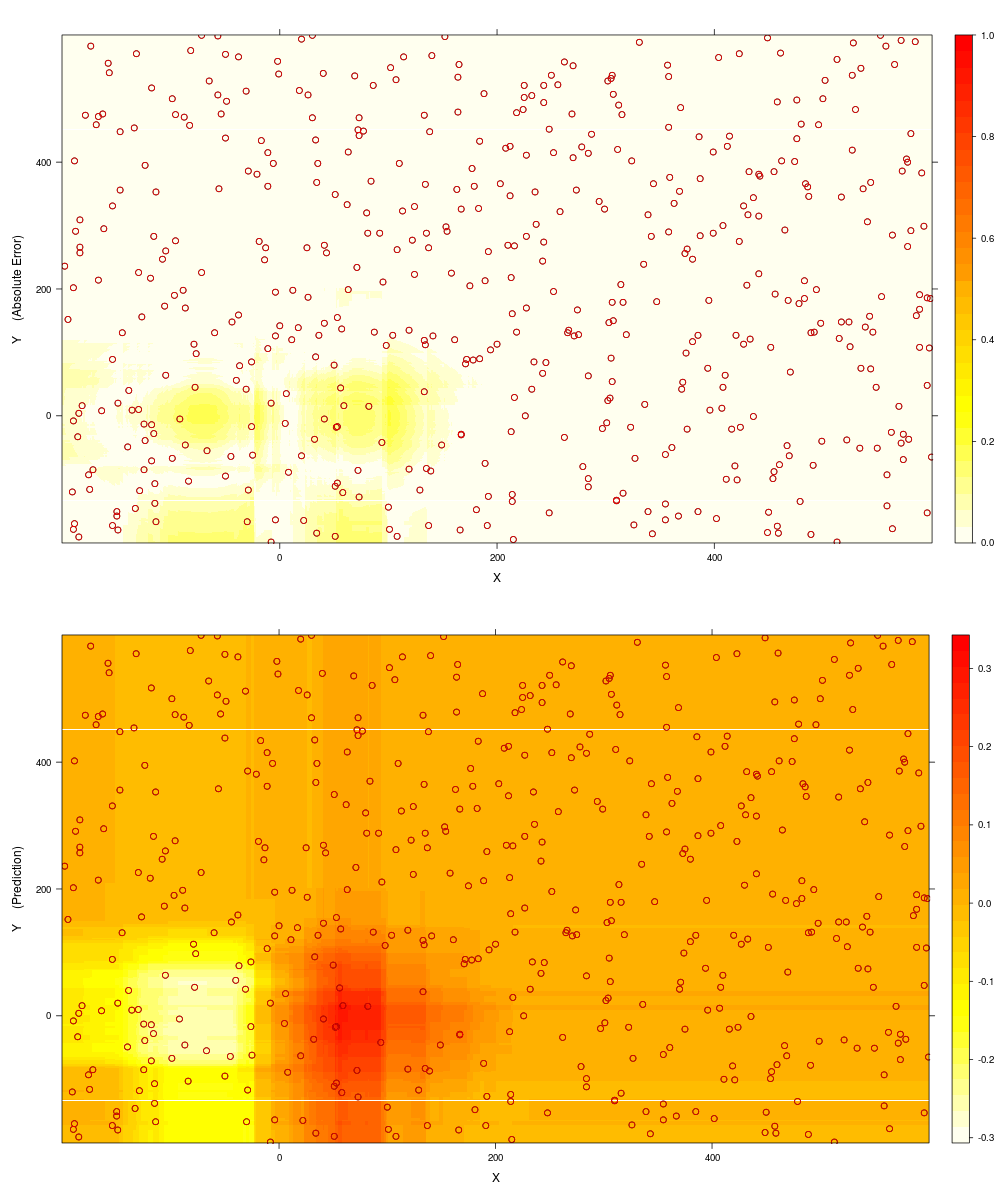
\includegraphics[width=\textwidth]{figures/ASK-first-plot.png}
\end{center}




